\documentclass[12]{article}
%\usepackage[utf8]{inputenc}
\usepackage{lmodern,textcomp}
\usepackage{hyperref}
\usepackage{graphicx}
\usepackage{float}
\usepackage[spanish]{babel}
%\usepackage{listings}


\title{Red Anónima I2P}
\author{Borja Fernández Merchán \\ Andrés Gomar Pérez \\ Carlos Rodrigo Sanabria Flores \\ Sergio Ruiz Pino
 \\ Iván Piña Arévalo}
\date{\today}

\section{�Qu� es un eepsite?}

Eepsites son sitios web en la red I2P, lo que significa https://es.overleaf.com/
project/5e1c7dac9592ed000175a9db que solo puede acceder a ellos con I2P. Las preguntas frecuentes oficiales dicen:

 Un eepsite es un sitio web alojado de forma an�nima, un servicio oculto al que se puede acceder a trav�s de su navegador web. Se puede acceder configurando el proxy HTTP de su navegador web para usar el proxy web I2P (normalmente escucha en el puerto local 4444) y navegando por el sitio.

Es f�cil configurar eepsites, pero no se puede conocer f�cilmente la direcci�n IP real de las eepsites. Los eepsites equivalen a los servicios ocultos de Tor.

Hay que tener en cuenta que los errores o defectos de dise�o en I2P o un descuido a�n pueden revelar la ubicaci�n accidentalmente.

\end{ }



\subsection{Manera f�cil: usar el servidor web I2P}

I2P viene con su propio servidor web basado en Jetty. Est� deshabilitado de forma predeterminada, pero se puede activar r�pidamente.

Ejecutamos I2P, accedemos a la consola del enrutador I2P (http:
//localhost:7657), luego hacemos clic en "T�NELES LOCALES" (o abrir directamente 
http://localhost:7657/i2ptunnelmgr). Ahora se puede ver el "ADMINISTRADOR DE SERVICIOS OCULTOS" y sepuede encontrar f�cilmente el "servidor web I2P" en "SERVICIOS OCULTOS DE I2P". Hacemos clic en el bot�n "Iniciar" en el lado derecho.

\begin{figure}
    \centering
    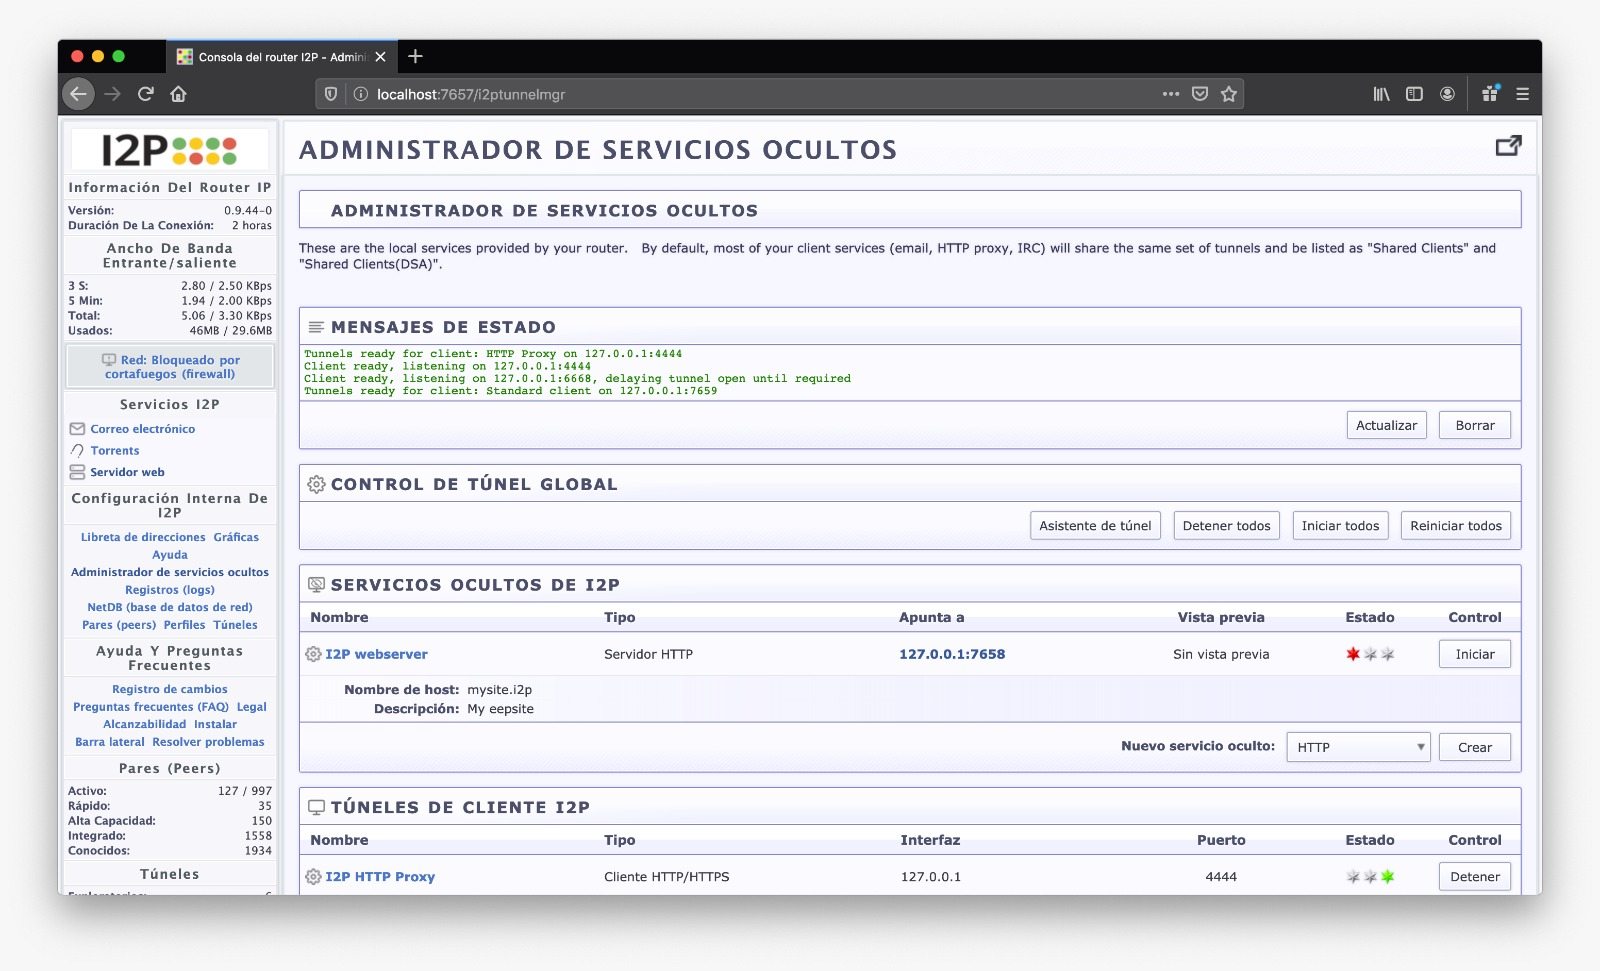
\includegraphics[width=\linewidth]{media/i2ptunnelmgr.jpeg}
    \caption{I2P Tunnel Manager}
    \label{fig1}
\end{figure}

Para visualizar la eepsite nos dirigimos a http://localhost:7658. Nos encontraremos la p�gina web predeterminada. Desafortunadamente, parte de la informaci�n en esa p�gina est� un poco anticuada.

\begin{figure}
    \centering
    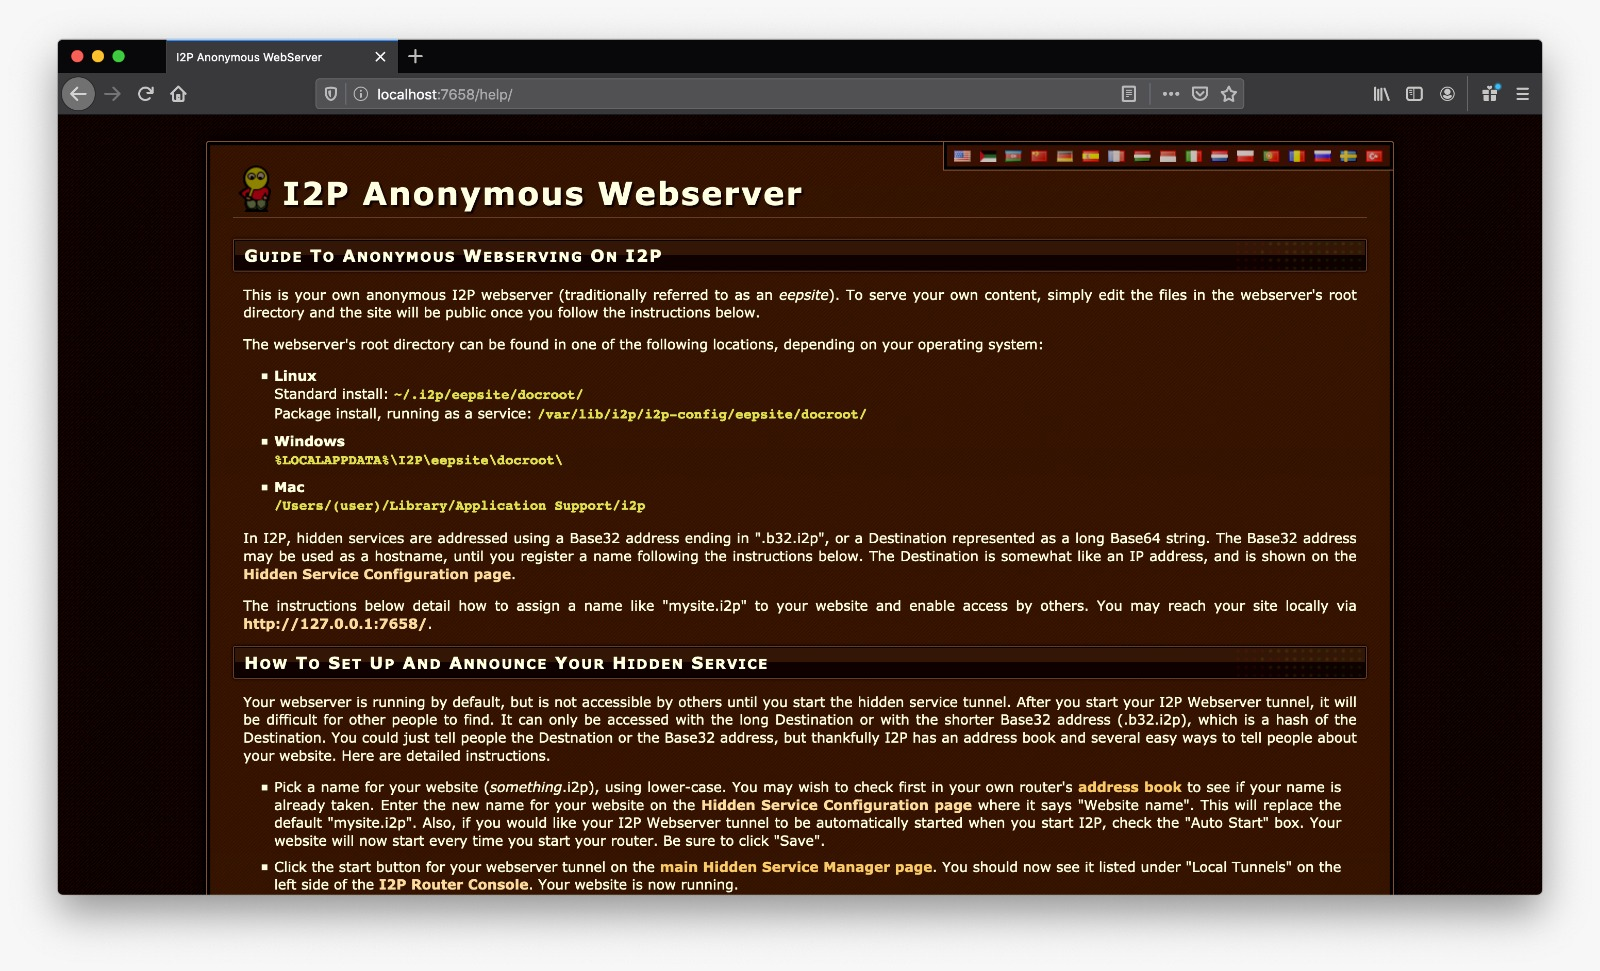
\includegraphics[width=\linewidth]{media/defaultpage.jpeg}
    \caption{Default Page}
    \label{fig2}
\end{figure}

Si solo desea configurar un blog est�tico simple, b�sicamente est� hecho. Se deben traladar los contenidos web a:

- Linux: `~/.i2p/eepsite/docroot/` o `/var/lib/i2p/i2p-config/eepsite/docroot/`
- Mac: `/Users/$USER/Library/Application Support/i2p`
- Windows: `%LOCALAPPDATA%\I2P\eepsite\docroot\`


\subsection{C�mo podemos acceder a nuestro eepsite?}

En primer lugar, las eepsite tienen "direcci�n" como una pagina web normal. Si se utiliza el servidor web I2P, se puede verificar la direcci�n haciendo clic en "Servidor web I2P" en "SERVICIOS OCULTOS I2P". Se encuentra en "Direcci�n local".

Por ejemplo la direcci�n de este sitio:

mhlKtPdwJ8
YmLQ-7r-3
xA1f8FWn
HMhWJ2rq
rvys7gS
vx1YM6KI
7gTa-K6
YPZGM2NP
XnHzTGz
DeGqTTU
gMCJ1Hz
R6305
dY1Tgf
cJQy1dk
8d
abKSss
L6NZff1
M
LFUoFmB
wHUBlk
Lj
GkD2y2
-2RedL
e-rMMO
M8PGPn
8u
3YYKMj
ViFzjkI
d8OJnX
Rj0tLK
9nyAgK
d36w6
MRC1JI
2MVOcF
S
-uurv
yekQ6
PKRqc1
saTYu
ohMUNO
RbEtY0
sb4Cp
evFTy
NRP-YrA
D7ckHr
0R8ydh
h~iVUG
M3RUIGH
dnVYzt
mS1F-3
ohx4ED
U1
3Kq20a
tkSN
QSUJS9
Xc
zAvE0r
CE1
IIqhRY
E
tPbQtm
ob-6
B0NTH7
oz
ib4WePH
c
eQZ8To
G
rnIurc
rS
oPGWXl
C
SLO~
yzGAv
5DD
M9c1p
XzH
t
YijY
JT1
j2i4u
MF
o1i
duJMv
lN
SPXxV
4B4r
FAFMw
Sa
ep-Nc
FFv
TiGX
gNu
TRAhO
DKH
6RcxB
w
2MFEM
BZ
0x
tO8L
p5
n~OD
28
Ty
GsM
I-V
JOwb
0BQ
AEAAc
AAA==

Sin embargo esta direcci�n es demaciado larga, podemos acortarla haciendo uso del siguiente script:

```py
#!/usr/bin/env python3
import base64, hashlib, sys

if len(sys.argv) != 2:
  print('Usage: convertkey.py <base64key>')
  sys.exit(1)

key =
sys.argv[1]
raw_key = 
base64.
b64decode
(key, '-~')
hash = 
hashlib.

sha256
(raw_key)
base32_hash
= base64

.b32encode
(hash.digest())
print
(base32_hash.
lower().

decode
("utf-8")
.replace
("=", "")
+ ".b32.i2p")
```

Al ejecutar el script obtenemos una direcci�n `.b32.i2p` como la siguiente:

trrfoanztrp25js6kmvqckc7khvntfgmjwvhdhqp5uxmw6yynkea.b32.i2p

Si metemos la url en un navegador con i2p nos debe redirigir a:


\begin{figure}
    \centering
    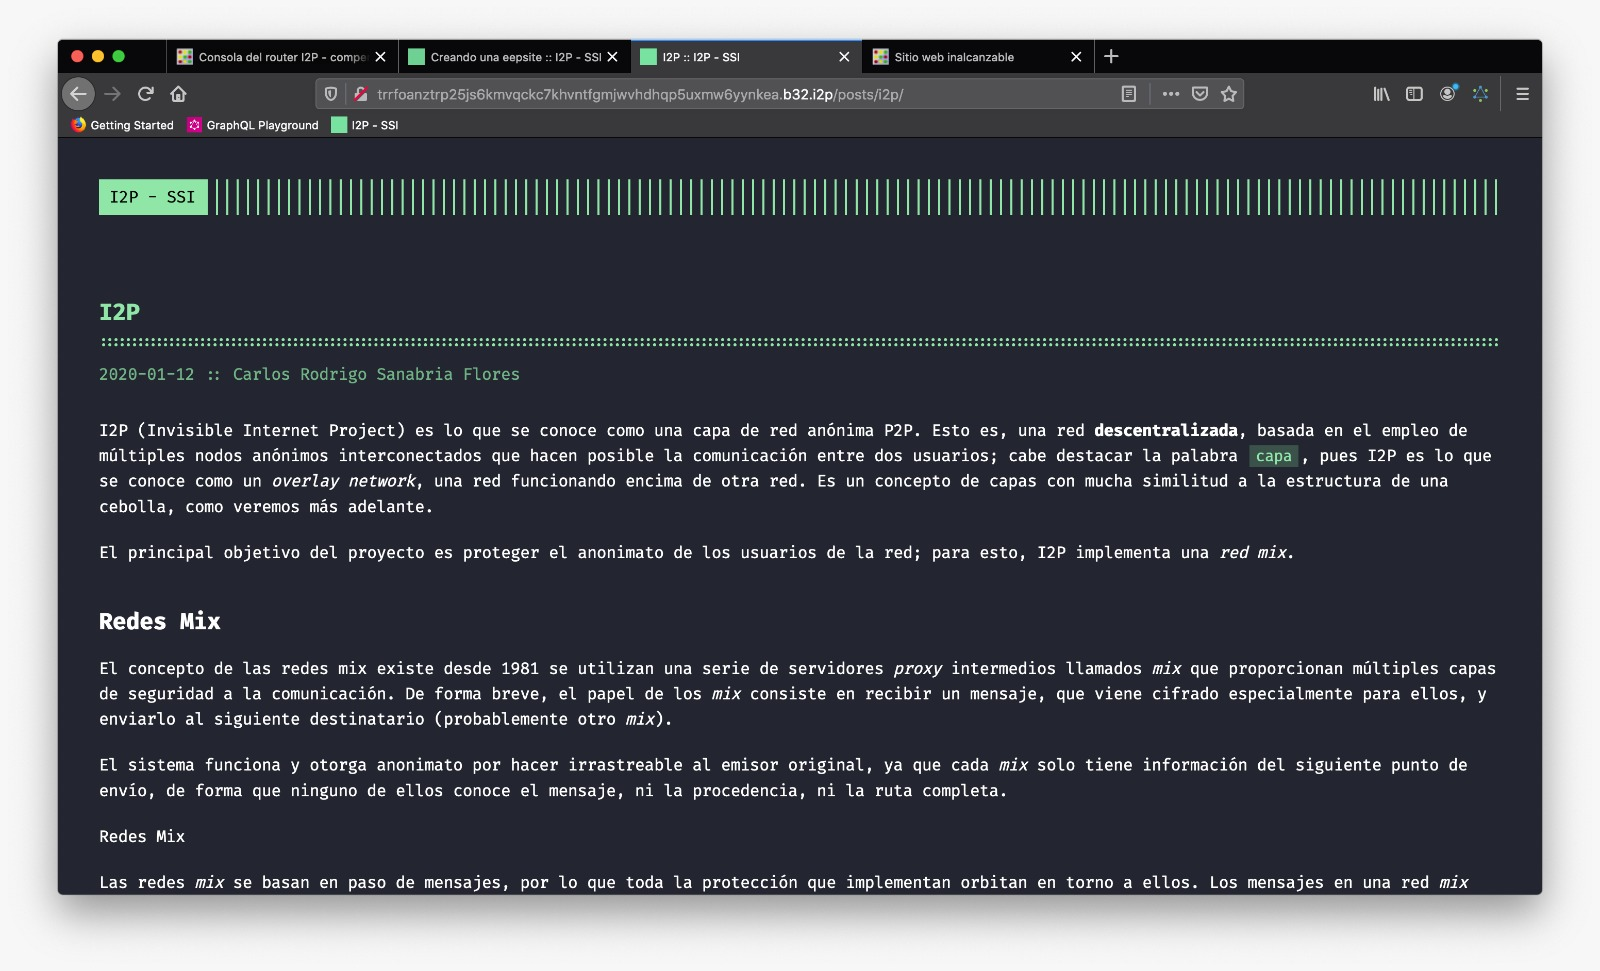
\includegraphics[width=\linewidth]{media/blog.jpeg}
    \caption{Blog}
    \label{fig3}
\end{figure}


\subsection{Creando una API oculta}


A diferencia del caso anterior esta vez utilizaremos nuestro propio servidor web para poder atender las peticiones para ello debemos congfigurar un nuevo servicio oculto, primero definimos el nombre del servicio, seleccionamos el puerto y por ultimo guardamos la configuracion.

\begin{figure}
    \centering
    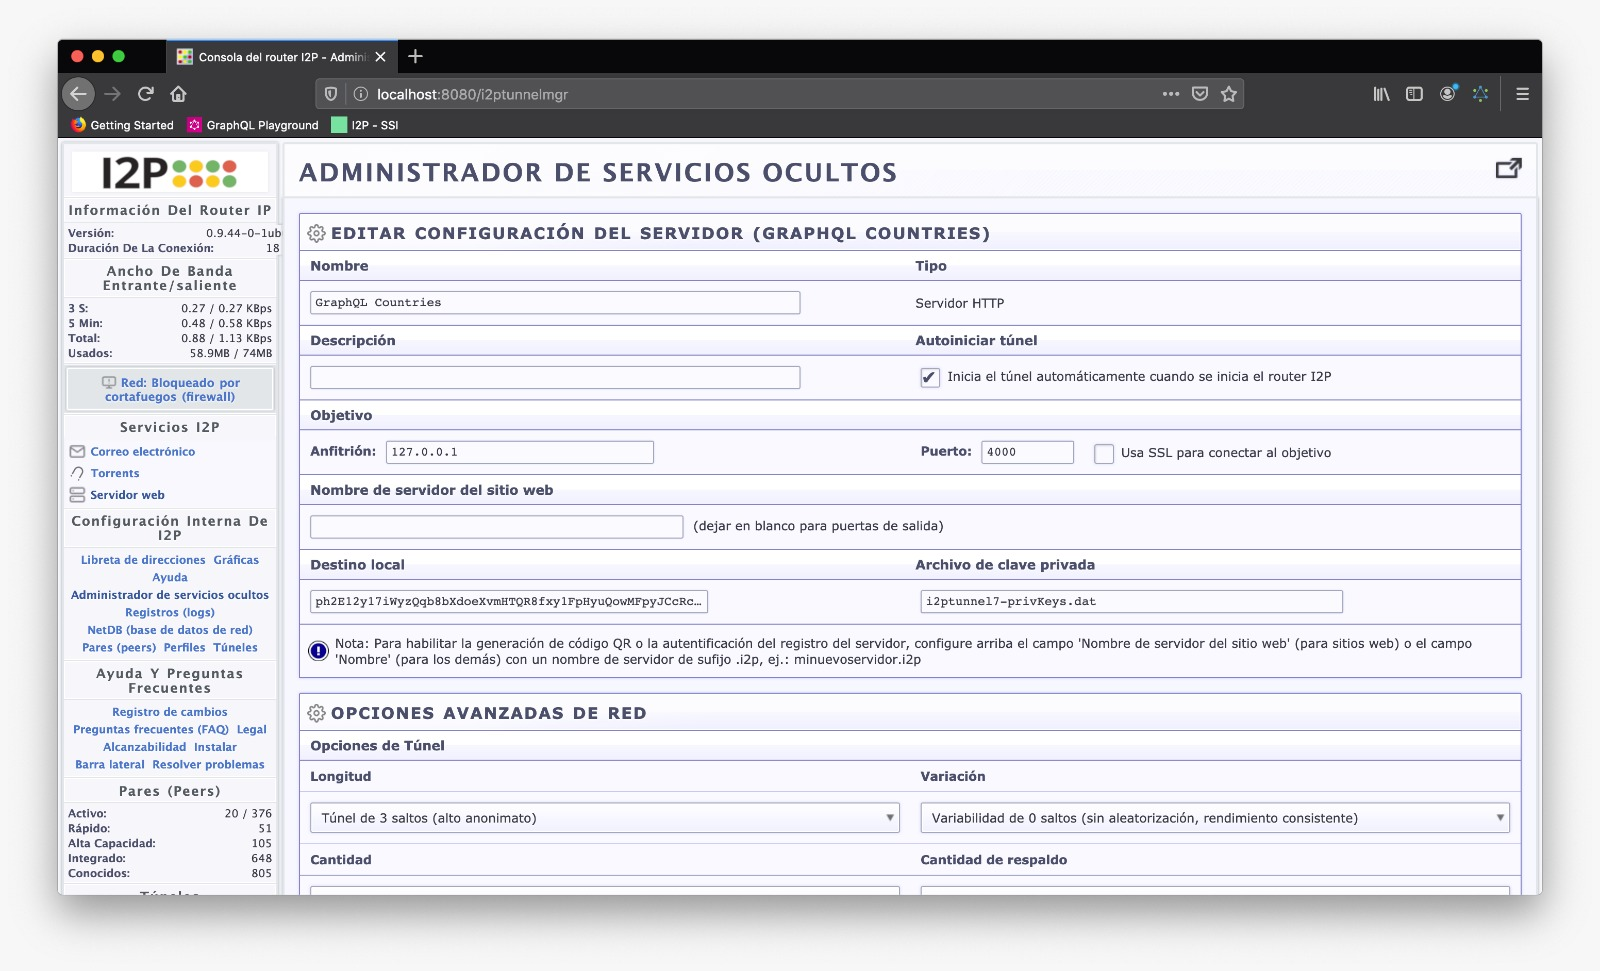
\includegraphics[width=\linewidth]{media/bindport.jpeg}
    \caption{Captura bindport}
    \label{fig4}
\end{figure}


finalmente obtenemos nuestra api disponible dentro de la red I2P:

\begin{figure}
    \centering
    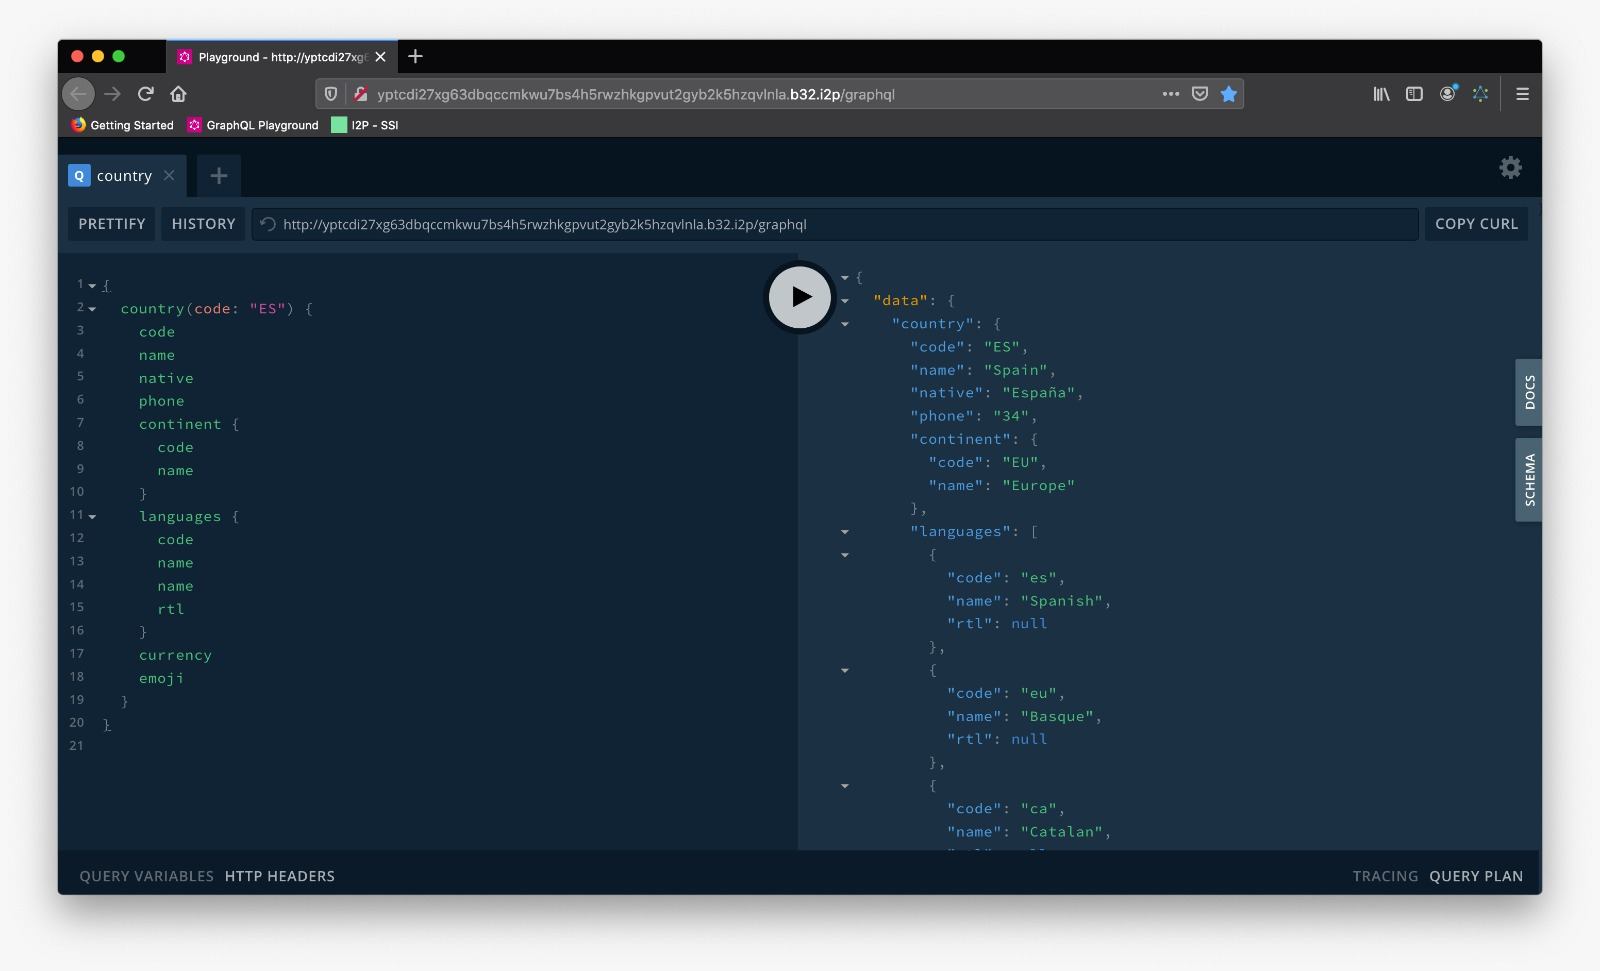
\includegraphics[width=\linewidth]{media/apigraphql.jpeg}
    \caption{Captura apigraphl}
    \label{fig5}
\end{figure}


\end{document}
